% HOMIE final-year project report. Compile with XeLaTeX (Overleaf) or Tectonic.
% All text, author details, tables and TikZ figures are editable.
\documentclass[12pt,a4paper,oneside]{report}
\usepackage[left=1.25in,right=1in,top=.75in,bottom=.75in,footskip=10mm]{geometry}
\usepackage[T1]{fontenc}
\usepackage{mathptmx}
\usepackage{graphicx,xcolor,booktabs,tabularx,array,amsmath}
\usepackage{float}
\usepackage{setspace,fancyhdr,titlesec,enumitem,tikz,caption}
\usetikzlibrary{arrows.meta,positioning}
\usepackage[hidelinks,hypertexnames=false]{hyperref}
\definecolor{institution}{RGB}{24,61,119}
\definecolor{rulecolour}{RGB}{112,70,31}
\newcommand{\ProjectTitle}{HOMIE: Machine Learning-Based Transaction Risk Assessment on Solana}
\newcommand{\AcademicYear}{2026--27}
\newcommand{\GuideName}{Mr. Manjunath Prasad}
\newcommand{\AuthorTable}{\begin{tabular}{ll}\textbf{Bharath Kumar Shetty}&4MT23AI013\\\textbf{Deepthi P. Salian}&4MT23AI017\\\textbf{Shreya Shetty}&4MT23AI051\\\textbf{Swaroop Nellitheertha}&4MT23AI056\end{tabular}}
\onehalfspacing
\setlength{\parindent}{0pt}
\setlength{\parskip}{4pt}
\setlength{\emergencystretch}{2em}
\setlist{nosep,leftmargin=*}
\setcounter{tocdepth}{1}
\pagestyle{fancy}\fancyhf{}
\fancyfoot[C]{\small Page \thepage}
\renewcommand{\headrulewidth}{0pt}\renewcommand{\footrulewidth}{0pt}
\fancypagestyle{plain}{\fancyhf{}\fancyfoot[C]{\small Page \thepage}}
\titleformat{\chapter}[display]{\centering\bfseries\fontsize{18}{22}\selectfont}{CHAPTER \thechapter}{10pt}{}
\titlespacing*{\chapter}{0pt}{8pt}{18pt}
\titleformat{\section}{\bfseries\fontsize{16}{20}\selectfont}{\thesection}{.7em}{}
\titleformat{\subsection}{\bfseries\fontsize{14}{17}\selectfont}{\thesubsection}{.7em}{}
\titlespacing*{\section}{0pt}{12pt}{6pt}
\titlespacing*{\subsection}{0pt}{10pt}{4pt}
\widowpenalty=10000\clubpenalty=10000
\captionsetup{font=small,labelfont=bf}
\newcolumntype{Y}{>{\raggedright\arraybackslash}X}
\newcommand{\CourseCode}{23AISE409}
\newcommand{\PageBorder}{\begin{tikzpicture}[remember picture,overlay]\draw[line width=.6pt] ([xshift=10mm,yshift=-10mm]current page.north west) rectangle ([xshift=-10mm,yshift=10mm]current page.south east);\end{tikzpicture}}
\newcommand{\Masthead}{{\fontsize{16}{19}\selectfont\bfseries MANGALORE INSTITUTE OF\par TECHNOLOGY \& ENGINEERING\par}\vspace{2mm}{\fontsize{9}{11}\selectfont (A Unit of Rajalaxmi Education Trust \textregistered, Mangalore)\par Autonomous Institute Affiliated to V.T.U, Belagavi, Approved by AICTE, New Delhi\par Accredited by NAAC with A+ Grade \& ISO 9001:2015 Certified Institution\par}}
\newcommand{\Department}{ARTIFICIAL INTELLIGENCE AND MACHINE LEARNING}
\renewcommand{\contentsname}{TABLE OF CONTENTS}
\renewcommand{\listfigurename}{LIST OF FIGURES}
\renewcommand{\listtablename}{LIST OF TABLES}
\begin{document}
\begin{titlepage}\PageBorder\centering\setstretch{1}\setlength{\parskip}{0pt}
\Masthead\vspace{4mm}
\includegraphics[height=28mm]{assets/mite_autonomous.jpeg}\par\vspace{4mm}
\textbf{PROJECT REPORT}\par\vspace{3mm}
\textbf{\CourseCode\ PROJECT PHASE -- II}\par\vspace{5mm}
{\fontsize{18}{22}\selectfont\bfseries ``HOMIE: MACHINE LEARNING-BASED TRANSACTION RISK ASSESSMENT ON SOLANA''\par}\vspace{5mm}
Submitted in partial fulfilment of the requirements for the award of the degree of\par\vspace{3mm}
\textbf{BACHELOR OF ENGINEERING}\par\vspace{2mm}in\par\vspace{2mm}
\textbf{\Department}\par\vspace{4mm}by\par\vspace{3mm}
\AuthorTable\par\vspace{6mm}
Under the Guidance of\par\textbf{\GuideName}\par
% Guide designation not supplied; leave unset.
\vspace{7mm}{\bfseries DEPARTMENT OF\par\Department\par}\par\vfill
\textbf{\AcademicYear}\par
\end{titlepage}
\pagenumbering{roman}
\begingroup\setstretch{1.15}\thispagestyle{empty}\PageBorder
\begin{center}\Masthead\vspace{5mm}
\includegraphics[height=28mm]{assets/mite_autonomous.jpeg}\par\vspace{4mm}
{\bfseries DEPARTMENT OF\par\Department\par}\par\vspace{8mm}
{\fontsize{18}{22}\selectfont\bfseries CERTIFICATE}\end{center}\vspace{5mm}
This is to certify that the Project Phase -- II (\textbf{\CourseCode}) work entitled \textbf{``\ProjectTitle''} is the project work carried out by the following students in partial fulfilment of the requirements for the award of the Bachelor of Engineering degree in Artificial Intelligence and Machine Learning at Mangalore Institute of Technology \& Engineering (Autonomous), affiliated to Visvesvaraya Technological University, Belagavi, during the academic year \AcademicYear.
\begin{center}\AuthorTable\end{center}
The report is submitted for examination under the guidance of \textbf{\GuideName}.
% Unsigned certificate form for institutional review and signatures.
\vspace{13mm}
\begin{tabularx}{\textwidth}{Y >{\raggedleft\arraybackslash}X}
\hrulefill&\hrulefill\\
\GuideName&Head of Department\\Project Guide&AI\&ML
\end{tabularx}
\vspace{15mm}\begin{center}\rule{45mm}{.4pt}\\Principal\end{center}
\clearpage\endgroup
\chapter*{DECLARATION}\thispagestyle{empty}\PageBorder
We declare that the Project Phase -- II (\CourseCode) report entitled \textbf{``\ProjectTitle''}, submitted in partial fulfilment of the requirements for the Bachelor of Engineering degree in Artificial Intelligence and Machine Learning, presents our project work carried out under the guidance of \textbf{\GuideName}. Sources of data, software and published research used in the work are acknowledged in the report. This report has not been submitted by us for the award of another degree.
\par\vspace{12mm}
\begin{tabularx}{\textwidth}{|c|Y|p{28mm}|}\hline
\textbf{Sr. No.}&\textbf{Name and USN}&\textbf{Signature}\\\hline
1&Bharath Kumar Shetty (4MT23AI013)&\\[5mm]\hline
2&Deepthi P. Salian (4MT23AI017)&\\[5mm]\hline
3&Shreya Shetty (4MT23AI051)&\\[5mm]\hline
4&Swaroop Nellitheertha (4MT23AI056)&\\[5mm]\hline
\end{tabularx}
\vspace{12mm}\par Place: Moodbidri\par Date: \rule{35mm}{.4pt}
\chapter*{ACKNOWLEDGEMENTS}\thispagestyle{empty}\PageBorder
We express our gratitude to our project guide, \GuideName, for guidance during Project Phase -- II. We thank the Head of Department, Principal and management of Mangalore Institute of Technology \& Engineering for providing the academic environment for this work. We also thank the faculty of the Department of Artificial Intelligence and Machine Learning for their support.

We acknowledge the maintainers of SolArchive for making blockchain records publicly accessible, and the developers of Solana, scikit-learn and the open-source tools used in the implementation. We thank our families and classmates for their encouragement and support.
\vspace{12mm}\begin{flushright}Bharath Kumar Shetty (4MT23AI013)\\Deepthi P. Salian (4MT23AI017)\\Shreya Shetty (4MT23AI051)\\Swaroop Nellitheertha (4MT23AI056)\end{flushright}
\chapter*{ABSTRACT}\thispagestyle{empty}\PageBorder
HOMIE assesses Solana transaction execution risk when the signer has no available outcome history. It constructs chronological features from public SolArchive records and compares histogram gradient boosting models with and without non-signer writable-account history. A one-hour outcome delay restricts features to earlier available labels. Both models also receive a learned identity score in the stronger comparison. On 17,904 reserved first-appearance transactions, average precision increases from 0.1688 to 0.2004; a further test on 19,515 transactions increases it from 0.2207 to 0.2393. The application supports historical replay, fitted-model inference, live transfer checks and decision-to-receipt recording. A local-validator experiment verifies that a landed execution failure can incur a fee while normal preflight can reject the same error without a fee. The results demonstrate additional historical failure-ranking signal; measured ML-driven fee savings are not claimed.
\par\vspace{4mm}\textbf{Keywords:} Solana, histogram gradient boosting, account history, transaction failure, temporal evaluation.
\tableofcontents\listoffigures\listoftables
\chapter*{ABBREVIATIONS / NOTATIONS}
\begin{tabularx}{\textwidth}{p{30mm}Y}\toprule Abbreviation&Meaning\\\midrule
AI&Artificial intelligence\\ML&Machine learning\\HGB&Histogram gradient boosting\\AP&Average precision\\AUROC&Area under the receiver operating characteristic curve\\FPR&False-positive rate\\TP / FP&True positive / false positive\\TN / FN&True negative / false negative\\RPC&Remote procedure call\\SOL&Native currency unit of Solana\\SGD&Stochastic gradient descent\\API&Application programming interface\\HTTP&Hypertext Transfer Protocol\\JSON&JavaScript Object Notation\\SQL&Structured Query Language\\CI&Confidence interval\\\bottomrule\end{tabularx}
\clearpage\pagenumbering{arabic}
\chapter{INTRODUCTION}
\section{Background}
HOMIE uses earlier Solana records to rank transactions by execution-failure risk. Transactions may transfer SOL or interact with blockchain programs.

A wallet may have no usable history in the collected sample. However, the accounts involved in its transaction may have appeared in other transactions. HOMIE uses these shared histories as additional input to a machine learning model. Here, an account is a blockchain data address; it does not necessarily represent another person's wallet.

\subsection{Wallets, signers and accounts}
A wallet helps a user manage signing keys and approve transactions. The signer is the address whose signature authorises a transaction. The primary signer used in this study is the first signer in the sampled record. A transaction may also reference accounts holding balances, program state or other data. These referenced accounts are not necessarily people or wallets~\cite{accounts,transactions}.

The distinction matters because the proposed model uses the history of \emph{participation} in transactions. If an account repeatedly appears in failed operations, that pattern may be informative about a later operation involving it. The model does not infer that the account owner caused those failures or acted maliciously.
\subsection{Writable and read-only account roles}
A writable account is declared as an account whose state may be changed by the transaction. A read-only account may be read without modification. These declarations describe access permissions, not a guarantee that an account will actually change. The project separates the primary signer from other writable accounts to avoid treating the signer's own history as new contextual evidence.

Read-only templates in this project are sets of declared read-only account addresses. They can capture recurring transaction contexts, but are not verified lists of programs invoked by each transaction. This definition follows the fields available in the selected archive.
\subsection{Failure, rejection and unknown outcome}
An execution failure is a recorded unsuccessful execution outcome. A candidate may instead be rejected before submission, or an attempted transaction may never appear in the observed archive. These cases must not be merged into the same label. The historical model is evaluated on included transactions with recorded outcomes. The application separately records simulation results and receipt availability.

\section{Problem Statement}
Signer-history models have little direct evidence when a signer has no available outcomes. The research question is: \emph{Does non-signer writable-account history improve failure ranking beyond transaction structure, signer history, read-only context and a learned identity control?}

\section{Motivation / Need for the Project}
A model that depends mainly on signer history can perform well on repeat participants while providing little information for a signer without earlier outcomes. Reporting only the aggregate score can hide this weakness. HOMIE therefore measures performance on a defined missing-history subgroup as well as examining the broader dataset.

Two subgroups are distinguished. A cold-history transaction has no matured primary-signer outcome available at its checkpoint. A first-appearance transaction is the first observed primary-signer occurrence in the sampled replay. A signer can appear repeatedly within the one-hour outcome delay and still remain cold. First-appearance evaluation reduces this particular source of repetition.

\section{Objectives}
\begin{enumerate}
\item Construct reproducible features from public transaction records using only earlier available outcomes.
\item Compare a baseline and a writable-context model on chronological test periods.
\item Evaluate first-appearance transactions separately from aggregate performance.
\item Implement a usable interface for inference, transfer checks and traceable outcome recording.
\item Verify the fee mechanism using an isolated local validator.
\end{enumerate}

\section{Scope of the Project}
HOMIE retains the name of the original DeFi-companion concept, but its implemented focus is transaction-risk assessment. The work contributes an empirical evaluation of account-context features and an integrated prototype. Histogram gradient boosting is an established algorithm; the research contribution is the feature comparison and evaluation setting, rather than a newly invented classifier.

The predicted label is execution failure, not fraud, malicious intent or investment risk. ``Cold history'' means unavailable signer outcomes in the sampled replay; it does not establish that a wallet is newly created on Solana.

\section{Significance and Expected Contribution}
Consider a signer with no available history that submits an operation referencing accounts A and B. Earlier transactions from other signers have involved these accounts. The baseline sees transaction structure and read-only context. The extended model additionally receives summaries of earlier outcomes involving writable A and B. It may assign a different score because these summaries supply evidence that the signer-only history lacks.

This example explains the mechanism; it is not an additional measured result. The model can increase or decrease a score depending on the learned pattern. A lower score alone does not prove an improvement. The recorded outcome and performance across the test set determine whether the predictions are useful.

\section{Organization of the Report}
Chapter 2 reviews relevant literature. Chapter 3 describes the proposed system, requirements and architecture. Chapter 4 explains the research methodology. Chapter 5 presents implementation and experimental verification. Chapter 6 reports results and analysis. Chapter 7 concludes the work and identifies future scope. References and a reproducibility appendix follow.

\chapter{LITERATURE REVIEW}
\section{Introduction}
This chapter reviews Solana execution studies, relational learning and the methodological foundations used in HOMIE.

\section{Review of Existing Work}
Zheng et al. study failed Solana transactions through large-scale measurements of initiators, programs and error patterns~\cite{zheng}. Their work establishes transaction failures as an empirical research subject. HOMIE focuses more narrowly on prediction when signer history is unavailable and on testing explicit shared-account history.

Solana's official documentation describes transaction fees and the RPC simulation interface~\cite{fees,simulation,send}. Simulation executes a candidate against a particular state; a statistical history model estimates patterns from past observations. These are different sources of information and require separate evaluation.

The scikit-learn histogram gradient boosting classifier provides the implemented tabular learning method~\cite{hgb}. Public SolArchive records supply the historical data~\cite{archive}.
\begin{table}[H]\centering\caption{Relationship between existing resources and HOMIE}
\small\begin{tabularx}{\textwidth}{p{32mm}YY}\toprule
Resource&Relevant contribution&HOMIE focus\\\midrule
Solana failure study&Characterisation of failed transactions&Prediction under missing signer history\\
Solana RPC simulation&Execution check against current state&Displayed alongside independent ML scores\\
Histogram gradient boosting&Established tabular classifier&Controlled account-history feature comparison\\
SolArchive&Public transaction archive&Chronological sampled evaluation\\\bottomrule\end{tabularx}\end{table}
\subsection{Temporal Relational Learning}
BRIGHT, proposed by Lu et al., addresses real-time fraud detection using graph neural networks~\cite{bright}. It explicitly prevents future transactions from sending information into predictions about earlier transactions and separates historical computation from real-time inference. The relevant lesson for HOMIE is the importance of an information boundary when relationships between entities are used as predictors.

HOMIE uses tabular participation summaries rather than a graph neural network. Its target is Solana execution failure rather than e-commerce fraud. BRIGHT is therefore related methodological work, not a directly evaluated baseline. No claim of outperforming BRIGHT is made because the datasets, labels and operating conditions differ.

\subsection{Boosting, Calibration and Evaluation}
Friedman formulates gradient boosting as stage-wise function approximation~\cite{friedman}. This provides the methodological foundation for building a predictor through successive corrections. HOMIE uses an existing histogram boosting implementation, so the algorithm is credited as established prior work rather than presented as the project's invention.

XGBoost by Chen and Guestrin describes a scalable tree-boosting system~\cite{xgboost}. LightGBM by Ke et al. develops efficient gradient boosted decision-tree training~\cite{lightgbm}. These are relevant alternatives in the tree-ensemble literature. The current study uses scikit-learn's histogram classifier; XGBoost and LightGBM results are not claimed as implemented comparisons. Their inclusion identifies the wider algorithm family and potential future benchmark alternatives.

Niculescu-Mizil and Caruana examine predicted probabilities and calibration across supervised learners~\cite{niculescu}. Their distinction between a discriminative score and a reliable probability motivates reporting calibration alongside ranking. HOMIE's isotonic follow-up is evaluated on chronological validation data and does not erase the need to inspect performance on later dates.

Saito and Rehmsmeier discuss precision--recall plots for imbalanced binary classification~\cite{saito}. The relevance is direct: failures form a minority of the reserved first-appearance group, and an always-success classifier would have high accuracy while missing every failure. Reporting AP, recall and false positives makes this trade-off visible.

Kapoor and Narayanan discuss leakage and reproducibility problems in ML-based science~\cite{leakage}. In HOMIE, chronology, delayed labels and exclusion of current execution outputs are safeguards against this class of error. These safeguards define what information the model can use; they do not replace external validation.

\begin{table}[H]\centering\caption{Methodological literature and its use in the project}
\small\begin{tabularx}{\textwidth}{p{30mm}YY}\toprule Work&Relevant concept&Use in HOMIE\\\midrule
Friedman~\cite{friedman}&Gradient boosting&Foundation of the fitted classifier\\
Chen and Guestrin~\cite{xgboost}; Ke et al.~\cite{lightgbm}&Efficient tree ensembles&Related methods, not claimed experiments\\
Weinberger et al.~\cite{hashing}&Feature hashing&Fixed-dimensional identity representation\\
Niculescu-Mizil and Caruana~\cite{niculescu}&Probability calibration&Separating ranking from numerical reliability\\
Saito and Rehmsmeier~\cite{saito}&Imbalanced evaluation&Precision--recall interpretation\\
Kapoor and Narayanan~\cite{leakage}&Leakage and reproducibility&Information-availability safeguards\\\bottomrule\end{tabularx}\end{table}

\section{Comparative Analysis}
\subsection{Signer-based prediction}
Signer history can summarise repeated behaviour efficiently. Its weakness in this study is absence of evidence for some signers at prediction time. Replacing missing history with a global average supplies a reasonable default but does not distinguish otherwise similar cold-history transactions. Shared-account features are tested as a way to add information in that setting.
\subsection{Identity-based learning}
A model may learn that particular addresses recur with particular outcomes. This can explain apparent benefits from contextual features. The identity-control experiment gives both compared models a score learned from role-tagged account identities, including writable identities. The remaining comparison asks whether explicit historical summaries help beyond that learned score.
\subsection{Execution simulation}
Simulation evaluates a candidate transaction against a network state. It can identify a concrete error without needing a statistical training set. Historical ML could be complementary if it captured useful residual information, but demonstrating that requires observations beyond a retrospective archive. HOMIE includes both mechanisms in the application while evaluating their findings separately.

\section{Research and Design Gap}
The tested hypothesis is that explicit writable-account participation summaries provide incremental ranking signal. A role-tagged identity learner is supplied to both compared models to make simple identity memorisation a stronger baseline. The positive results support this bounded empirical contribution; they do not establish universal novelty across all blockchain prediction research.

\section{Summary}
The report addresses three questions. First, does writable context improve failure ranking for sampled cold-history transactions? Second, does the improvement remain for first appearances when both models receive an identity score? Third, what happens when historical scores are turned into practical warning policies?

Chronological experiments address the first two questions. Calibration and a cost audit address the third, with fee behaviour verified separately on a local validator.

\chapter{PROPOSED SYSTEM AND SCOPE}
\section{Problem Formulation}
Signer-history models have little direct evidence when a signer has no available outcomes. The research question is: \emph{Does non-signer writable-account history improve failure ranking beyond transaction structure, signer history, read-only context and a learned identity control?}

\section{Proposed Solution}
HOMIE combines a historical ML comparison with a transfer-checking application. The extended model adds writable-account participation history to the baseline. Network checks and recorded outcomes are displayed separately from model scores.

\section{Requirements}
\subsection{Functional and Non-Functional Requirements}
The system must support historical replay, fitted-model inference, public-history refresh, native SOL transfer checks and outcome recording. It must report whether data is fresh enough for live scoring. It must preserve the exact candidate message and model provenance before associating a later receipt with a decision.

Insufficient or stale live history must withhold an ML score. Missing network responses must remain incomplete checks. Unknown receipt outcomes must remain unknown. The web application performs checks without signing or broadcasting transactions.


The live flow accepts the selected network, sender address, recipient address and transfer amount. Addresses must be valid public keys. Amounts are parsed exactly into lamports; arbitrary floating-point rounding must not alter the intended transfer. The supported candidate is a plain native SOL transfer. Arbitrary token swaps and multi-instruction DeFi transactions are outside this implemented checker.

Outputs include a clear current-network finding, the quoted fee, the amount-plus-fee requirement and any balance shortfall. When valid history and model artifacts are available, the response also contains actual model scores and provenance. It records whether simulation occurred and whether signature verification was enabled. Each saved observation has an identifier for later lookup.

\subsection{Hardware and Operating Requirements}
Historical experiments require local storage for selected archive data and sufficient memory for feature tables. Live checks require an Internet connection and an available RPC endpoint. A browser and the Python environment run the application; local fee verification additionally requires a Solana validator installation. Minimum hardware throughput has not been benchmarked, so no unsupported minimum performance guarantee is specified.

\subsection{Software Requirements}
\begin{table}[H]\centering\caption{Implemented technology stack}
\begin{tabularx}{\textwidth}{p{38mm}Y}\toprule Component&Technology and purpose\\\midrule
Data processing&Python, pandas~\cite{pandas}, NumPy~\cite{numpy} and PyArrow for archive extraction and features\\
Machine learning&scikit-learn~\cite{sklearn} histogram gradient boosting; SGD logistic identity control; isotonic calibration follow-up\\
Backend&FastAPI served with Uvicorn\\
Interface&Browser-based HTML, CSS and JavaScript\\
Study storage&SQLite for immutable decisions and separately attached receipts\\
Blockchain access&Solana JSON-RPC for blocks, balances, fee quotes and simulation\\
Verification&pytest and an isolated Solana local validator\\\bottomrule\end{tabularx}\end{table}

\section{System Architecture / Block Diagram}
The architecture separates historical experimentation from live transfer analysis. Both routes reuse participation-history features, but live scores are experimental because current sampling and network conditions differ from the historical training data.
\begin{figure}[H]\centering\includegraphics[width=\textwidth,height=.70\textheight,keepaspectratio]{assets/architecture.png}\caption{Implemented research and application architecture.}\end{figure}
\subsection{Transaction-Check Workflow}
\begin{figure}[H]\centering
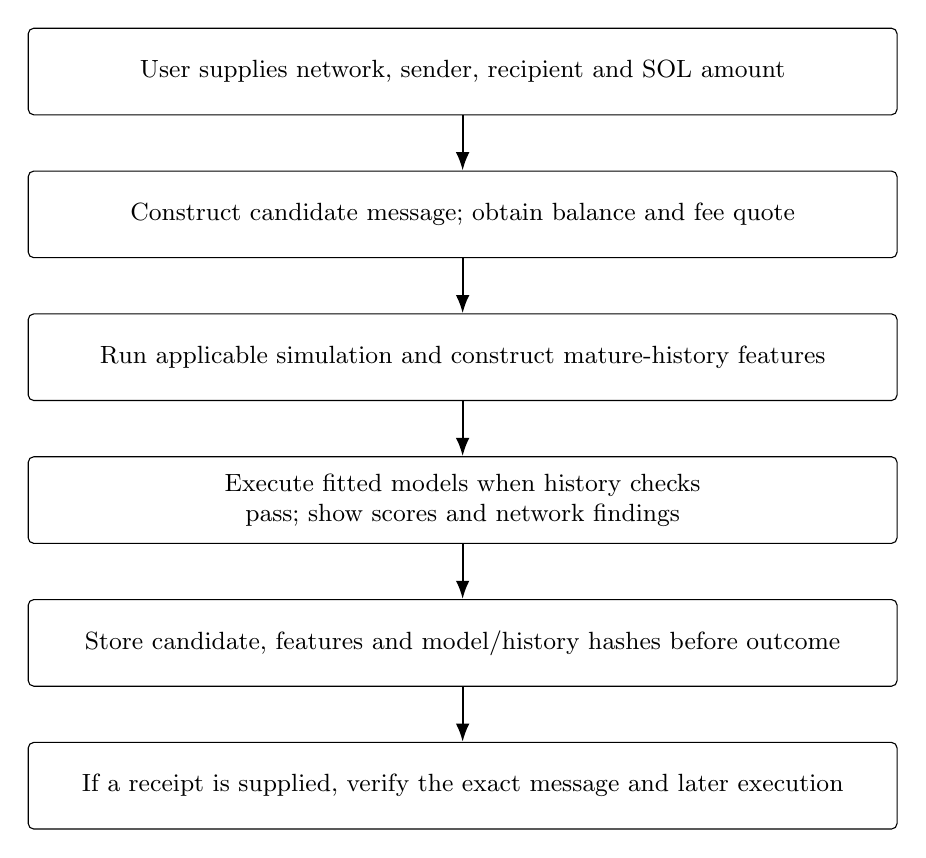
\begin{tikzpicture}[node distance=7mm,box/.style={draw,rounded corners=2pt,align=center,text width=108mm,minimum height=11mm,font=\small},arr/.style={-{Latex},thick}]
\node[box](a){User supplies network, sender, recipient and SOL amount};
\node[box,below=of a](b){Construct candidate message; obtain balance and fee quote};
\node[box,below=of b](c){Run applicable simulation and construct mature-history features};
\node[box,below=of c](d){Execute fitted models when history checks pass; show scores and network findings};
\node[box,below=of d](e){Store candidate, features and model/history hashes before outcome};
\node[box,below=of e](f){If a receipt is supplied, verify the exact message and later execution};
\foreach \x/\y in {a/b,b/c,c/d,d/e,e/f}\draw[arr](\x)--(\y);
\end{tikzpicture}\caption{Live checking and outcome-recording workflow.}\end{figure}

\subsection{Data and Responsibility Boundaries}
The archive provides transaction outcomes for retrospective evaluation. The RPC service supplies present network observations. The ML component consumes account-role and historical features; transfer amount is handled by the balance and simulation checks. The study store preserves the decision before the receipt is attached. This separation makes it possible to identify which component produced each finding.

\section{Functional / System Components}
\begin{table}[H]\centering\caption{Implemented modules and responsibilities}
\small\begin{tabularx}{\textwidth}{p{36mm}YY}\toprule Module&Input&Responsibility\\\midrule
Archive extraction&Selected date and shard&Retrieve selected columns and record provenance\\
Participation history&Chronological account roles and matured labels&Produce structural and contextual features\\
Model training&Training and validation feature tables&Fit controlled classifiers and retain artifacts\\
Live history&Public RPC blocks&Prepare network-specific mature snapshots\\
Transfer checker&Addresses, amount and network&Construct message; check balance, fee and simulation\\
Study store&Decision payload and later signature&Preserve observation; verify matching receipt\\
Web interface&User selection or transfer input&Display results and inspection links\\\bottomrule\end{tabularx}\end{table}

\begin{table}[H]\centering\caption{Users and supported activities}
\begin{tabularx}{\textwidth}{p{29mm}YY}\toprule User&Activity&System output\\\midrule
Researcher&Compare baseline and context predictions&Metric tables, saved predictions and provenance\\
Project evaluator&Inspect a historical example&Features, model scores and revealed recorded result\\
Transfer user&Check a proposed native SOL transfer&Balance, fee quote, simulation finding and experimental score\\
Study operator&Link a later transaction receipt&Verified matching outcome or explicit rejection\\\bottomrule\end{tabularx}\end{table}

\section{Scope and Constraints}
The historical workflow records extraction settings and derived-file hashes. Conflicting records or date mismatches must not be silently repaired into convenient data. Training, validation and test boundaries are defined chronologically. Feature columns and model settings are retained so exported inference consumes the same type and order of inputs used during fitting.

The live collector and model scorer must agree on the network. A mainnet-trained experiment may be inspected on devnet for functional testing, but devnet output is not evidence of equivalent predictive performance. A snapshot's collection timestamp and the maturity of its rows are checked separately.

The interface provides concise findings with inspectable evidence. Separate modules support collection, inference, transfer checks and receipt storage.


Invalid inputs are rejected before RPC calls. Unavailable RPC or history data produces an explicit incomplete result. Receipts must match the checked message; a changed blockhash requires a new observation.

\chapter{METHODOLOGY}
\section{Objective of the Study}
The study tests whether writable-account history adds failure-ranking information when signer history is unavailable, including a stronger comparison with a shared identity score.

\section{Method / Approach}
The historical source is SolArchive, licensed CC BY 4.0~\cite{archive}. The pinned dataset revision is:\par
{\small\texttt{6588cad2832e62be03972ac80d69c6af11d631c8}}\par
 One selected Parquet row group per date is used. The initial four windows contain 1,588,408 raw records before duplicate removal and exclusions. This is a sparse sample, not complete chain coverage.

Selected fields include transaction signature, account addresses and roles, block timestamp, block slot and execution status. The target is binary execution failure. Original instruction payloads, unlanded attempts and paid fee amounts are not available in the selected historical table.

\section{Measurement / Evaluation Parameters}
\begin{table}[H]\centering\caption{Chronological experimental windows (2025)}
\begin{tabular}{llll}\toprule Window&Training&Validation&Testing\\\midrule Initial&Nov. 1&Nov. 2&Nov. 3\\Confirmation&Nov. 8&Nov. 9&Nov. 10\\Extension&Nov. 22&Nov. 23&Nov. 24\\Reserved refined&Nov. 29&Nov. 30&Dec. 1\\Further test&Dec. 3&Dec. 4&Dec. 5\\\bottomrule\end{tabular}\end{table}
Average precision (AP) measures how well failures rank ahead of successful transactions across score cut-offs. It is not classification accuracy. AUROC, Brier loss, recall and false-positive rate provide complementary information. Paired bootstrap resampling of hourly blocks uses 500 draws to estimate uncertainty in AP differences.

\subsection{Metrics and interpretation}
Let TP denote flagged failures, FP flagged successes, FN missed failures and TN unflagged successes. For a fixed warning threshold,
\begin{align}
\mathrm{Precision}&=\frac{TP}{TP+FP}, &\mathrm{Recall}&=\frac{TP}{TP+FN},\\
\mathrm{FPR}&=\frac{FP}{FP+TN}, &\mathrm{Accuracy}&=\frac{TP+TN}{TP+FP+FN+TN}.
\end{align}
A classifier that always predicts success has accuracy equal to the success prevalence. On the reserved first-appearance group with 5.88\% failures, that simple rule would have about 94.12\% accuracy but identify no failures. This is why accuracy alone is unsuitable for judging the research question. Precision--recall analysis is particularly informative for imbalanced binary tasks~\cite{saito}.

Average precision summarises the precision--recall curve as $\sum_k(R_k-R_{k-1})P_k$, where $P_k$ and $R_k$ are precision and recall as the score threshold changes~\cite{ap}. AUROC describes ranking across positive and negative cases. Brier loss, $N^{-1}\sum_i(s_i-y_i)^2$, assesses the numerical predictions against binary outcomes; lower values are better~\cite{brier}.
\subsection{Uncertainty and experimental discipline}
The paired-hour bootstrap samples hourly blocks and computes the difference between both models on the same resampled observations. Pairing preserves their direct comparison. Grouping by hour accounts for some temporal clustering rather than treating every transaction as independent. The resulting interval is conditional on the fitted models and sampled periods; it does not measure all possible deployment uncertainty.

The reserved refined endpoint was specified after earlier exploratory diagnostics and before inspecting the fourth window's outcomes. It is a reserved historical test, not a publicly preregistered live trial. The further December window supplies another chronological comparison. This distinction makes the development of the research question clear without presenting exploratory choices as fixed from the start.

\section{Tools, Equipment and Resources}
Python, pandas, NumPy and PyArrow prepare chronological tables. Scikit-learn fits classifiers and computes metrics. Public SolArchive data supports the historical study; a Solana local validator supports the separate fee experiment.

\section{Experimental Procedure}
The research path transforms archive records into a feature table, then into fitted models and held-out predictions. Test labels are used to evaluate those predictions and to update later history only after the defined delay. They are not used to refit the gradient boosting model during the test day.
\begin{figure}[H]\centering
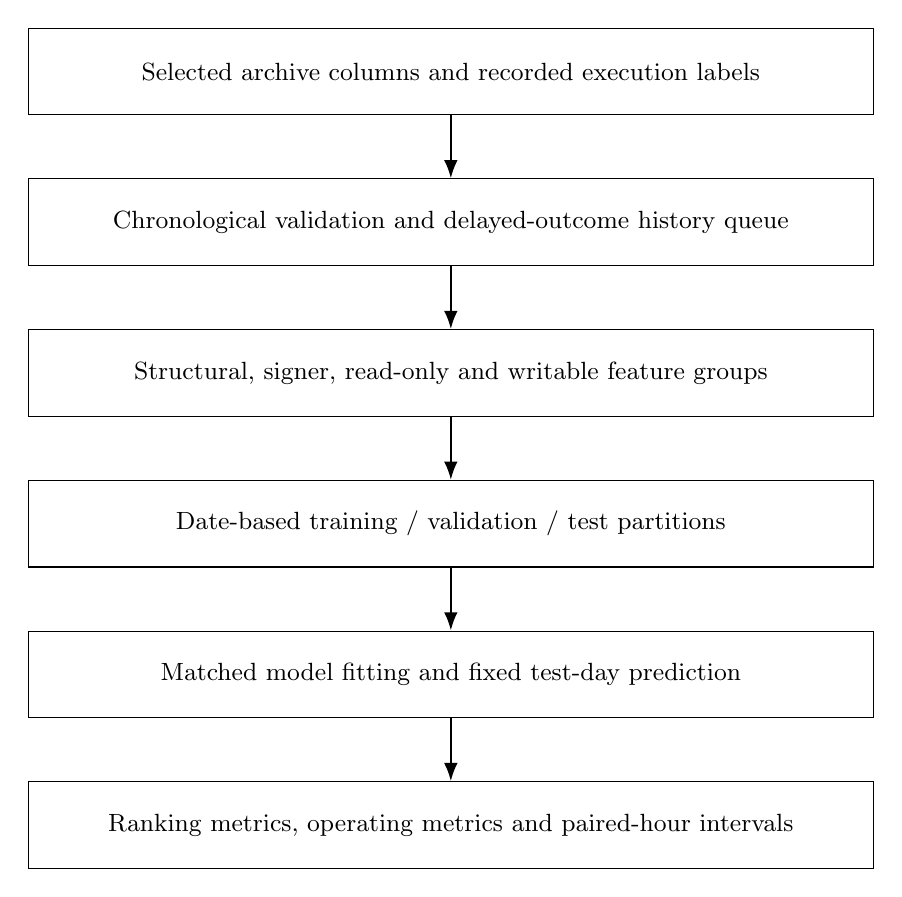
\begin{tikzpicture}[node distance=8mm,b/.style={draw,align=center,text width=105mm,minimum height=11mm,font=\small},a/.style={-{Latex},thick}]
\node[b](a){Selected archive columns and recorded execution labels};
\node[b,below=of a](b){Chronological validation and delayed-outcome history queue};
\node[b,below=of b](c){Structural, signer, read-only and writable feature groups};
\node[b,below=of c](d){Date-based training / validation / test partitions};
\node[b,below=of d](e){Matched model fitting and fixed test-day prediction};
\node[b,below=of e](f){Ranking metrics, operating metrics and paired-hour intervals};
\foreach \x/\y in {a/b,b/c,c/d,d/e,e/f}\draw[a](\x)--(\y);
\end{tikzpicture}\caption{Historical research data flow.}\end{figure}

\section{Model Architecture}
Histogram gradient boosting combines successive decision trees to reduce classification loss, following the gradient boosting framework~\cite{friedman}. Numeric feature values are grouped into bins for efficient split selection~\cite{hgb}. Both primary models use the same classifier settings so the comparison concerns the added features.
\begin{table}[H]\centering\caption{Histogram gradient boosting configuration}
\begin{tabular}{ll}\toprule Parameter&Value\\\midrule Maximum iterations&150\\Maximum leaf nodes&15\\Minimum samples per leaf&40\\L2 regularisation&5\\Early stopping&Disabled\\Seeds averaged&42, 73, 101\\\bottomrule\end{tabular}\end{table}
The fits are effectively deterministic; the three seeds are not independent experimental replications. The baseline includes structure, signer history and read-only/template history. The context model adds non-signer writable-account history.

\subsection{How boosting produces a score}
The classifier learns a sequence of trees. Each new tree contributes a correction to the model's current decision function. In binary classification, the decision function $z(x)$ is mapped to a score through a logistic link:
\begin{equation}z_M(x)=z_0+\eta\sum_{m=1}^{M}h_m(x),\qquad s(x)=\frac{1}{1+e^{-z_M(x)}}.\end{equation}
Here $h_m$ is a fitted tree and $\eta$ is the learning-rate parameter. Training reduces binary log loss, which penalises confident incorrect predictions. A probability-shaped output from this function still requires calibration assessment before being interpreted as an accurate event frequency in a new population.
\subsection{Why a tabular model fits this implementation}
The input is a fixed-length numeric representation of transaction structure and account history. A tree ensemble can learn non-linear combinations, such as different effects of a historical rate at low and high observation counts. It does not require a sequence of natural-language queries or a language model. The implemented method also allows a controlled feature ablation with the same learner on both sides.

Deep learning and graph models are possible extensions, but their inclusion would require a defined representation, training procedure and fair comparison. They are not necessary to describe the actual implemented contribution. The report therefore identifies histogram gradient boosting as the main algorithm and distinguishes the logistic identity control from it.

\subsection{Identity Control and Calibration}
A stronger comparison uses an SGD logistic learner~\cite{sgd} with role-tagged identities and read-only templates hashed into $2^{20}$ dimensions. Feature hashing provides a fixed-dimensional representation of large categorical spaces~\cite{hashing}. Binary features are L2 normalised; regularisation is 0.0001. Its chronological predictions are supplied to both gradient boosting models. Labels mature after one hour, with ten-minute learning batches introducing a small additional update delay.

A separate operational follow-up fits isotonic calibration~\cite{isotonic,niculescu} on early cold-history validation data and chooses thresholds on later validation data. This follow-up is distinct from the identity-controlled primary comparison. Live application outputs remain experimental raw scores rather than validated live failure probabilities.

\section{Error Sources and Mitigation}
Temporal leakage, repeated signers and identity memorisation can distort an apparent improvement. Delayed labels, a first-appearance endpoint and a shared identity control address these risks. Sparse sampling and changing network conditions remain limits of the evaluation.

\section{Data Processing and Analysis}
At transaction time $t$, an earlier outcome contributes only if its inclusion timestamp is at least one hour earlier. Features are computed before the current outcome is scheduled for later availability. The first six training hours build history. Rows whose labels would cross the next date boundary are purged from training and validation.

For account $a$ in role $r$, the smoothed historical failure rate is
\begin{equation}q_r(a,t)=\frac{f_r(a,t)+20b(t)}{n_r(a,t)+20},\qquad b(t)=\frac{F(t)+1}{N(t)+2}.\end{equation}
Here $f_r$ and $n_r$ are available failures and observations for that role; $F$ and $N$ are their global counterparts. Features summarise seen fractions, log counts and failure-rate mean, maximum, minimum and standard deviation. Ten common infrastructure addresses are excluded from contextual histories and represented through structural indicators.

\subsection{Worked history example}
Suppose an account has participated in ten matured observations, including two failures, and the global available failure rate is 0.05. With smoothing strength 20, its rate is
\begin{equation}q=\frac{2+20(0.05)}{10+20}=0.10.\end{equation}
With no account observations, the same rule returns the global rate. This avoids assigning an extreme rate to an account solely because one observed transaction failed. The example uses illustrative counts to explain the implemented formula; it is not a result sampled from the evaluation.
\subsection{Feature groups}
\begin{table}[H]\centering\caption{Feature groups and their interpretation}
\small\begin{tabularx}{\textwidth}{p{29mm}YY}\toprule Group&Examples&What it describes\\\midrule
Structure&Account, signer and writable counts; duplicates&Declared transaction composition\\
Signer history&Smoothed failure rate and log count&Available outcomes for the primary signer\\
Read-only history&Seen fraction, counts and rate summaries&Prior participation of read-only accounts\\
Read-only template&Template rate and count&Recurring declared account set\\
Writable history&Seen fraction and rate/count summaries&Prior participation of non-signer writable accounts\\
Infrastructure&Presence indicators&Common infrastructure accounts without pooled context histories\\\bottomrule\end{tabularx}\end{table}
Seen fraction is a coverage measure: a value of 14.3\% means that proportion of the relevant accounts has earlier available observations. It is not an accuracy score or a failure probability. The failure rates and coverage variables give the model both a pattern and information about how much history supports it.
\subsection{Leakage prevention}
Using the current transaction's error message would make failure prediction trivial after execution. Leakage of unavailable information can invalidate an ML evaluation~\cite{leakage}. HOMIE therefore excludes current logs, errors, consumed compute, balances, paid fees and block position from its historical model inputs. Time controls chronology and information availability but is not supplied as a numeric predictor.

Consider a transaction included at 10:20. Under the study's one-hour delay, its label cannot contribute to a 10:45 prediction. It becomes eligible at 11:20. The delay is an explicit research assumption. Inclusion timestamps do not reconstruct the exact information available at historical submission time.
\subsection{Replay procedure}
For each chronological record, the feature builder first releases eligible earlier labels from the pending queue. It then resolves the current account roles and computes features from that available history. Only after the feature row is produced is the current outcome scheduled for release one hour later. This order is reused across the research and live-history extraction paths.

\chapter{IMPLEMENTATION AND EXPERIMENTAL WORK}
\section{Implementation Environment}
The application uses FastAPI and Uvicorn, browser-based HTML, CSS and JavaScript, and SQLite for observation storage. Research outputs and fitted model artifacts are loaded from the project workspace.

\section{Module-wise Implementation}
The FastAPI application~\cite{fastapi} provides historical replay at \texttt{/}, fitted inference at \texttt{/predict}, transfer checks at \texttt{/check}, integrated analysis at \texttt{/live} and fee verification at \texttt{/fee-proof}. The backend reconstructs plain SOL transfer messages, handles exact lamport amounts and queries Solana RPC. It obtains a recent blockhash~\cite{blockhash}, requests a fee quote for the constructed message~\cite{feequote} and reads the sender balance~\cite{balance}.

Live snapshots must meet freshness and history requirements: at least 100 records spanning six hours, with a snapshot no older than one hour. Public blocks are retrieved using the documented block RPC~\cite{getblock}. Only outcomes aged at least one hour enter history. The same extractor used in research builds live features. Scores are withheld when checks fail.

SQLite records candidate-message, feature, model and history hashes. Database triggers protect decisions and receipts from mutation. Receipt verification checks the exact candidate message, signature, later slot and timestamp, and consistency of fee and balance changes. The receipt is retrieved through the transaction RPC~\cite{gettransaction}. An unrelated receipt cannot be used as evidence for a decision.

\subsection{Balance, fee and amount calculation}
For balance $B$, requested amount $A$ and quoted fee $F$, the checker calculates
\begin{equation}\mathrm{required}=A+F,\qquad \mathrm{shortfall}=\max(0,A+F-B).\end{equation}
For example, if a recorded check has a balance of 0.5120009 SOL, a requested transfer of 1 SOL and a quoted fee of 0.000005 SOL, the shortfall is 0.4880041 SOL. This corresponds to the saved insufficient-balance verification case. A sufficient balance passes this arithmetic check but may still encounter a separate simulation error.
\subsection{Simulation modes}
The standard web check creates an unsigned candidate and calls simulation with signature verification disabled. This allows a user to inspect supported execution conditions without supplying a private key. The result concerns the candidate at the checked state, not whether a valid signature will later be provided.

A separate signed-observation route accepts an already signed plain transfer, preserves its blockhash and enables signature verification during simulation. It still does not submit the transaction. The two modes are labelled separately because an unsigned check and signed simulation do not establish the same facts.
\subsection{Model provenance and range checks}
The stored response includes hashes identifying the model artifact, history snapshot and feature values. These support later inspection of which inputs produced the score. Live input values are compared with central training ranges as a diagnostic. A value within those ranges is not proof that a new transaction has the same outcome distribution as the training set.

Changing the amount may change the balance or simulation finding while leaving the ML score unchanged, because the current ML features do not encode the amount. This behaviour follows the feature definition and is useful to explain during a demonstration. The model assesses account context; the network checker assesses the constructed amount-specific candidate.

\subsection{Decision Storage}
The implemented SQLite store uses a decision table, a receipt table and an abstention table. SQLite triggers support rejecting updates and deletions of protected records~\cite{sqlite}. A decision has a generated identifier, serialised payload, payload hash and recording timestamp. The payload contains the candidate and the relevant check and model observations. Receipts are stored separately so a later outcome cannot overwrite what was known at prediction time.
\begin{table}[H]\centering\caption{Study-store entities}
\small\begin{tabularx}{\textwidth}{p{25mm}YY}\toprule Entity&Main fields&Relationship or constraint\\\midrule
Decisions&id, payload, payload hash, recorded time&Primary record; update and delete triggers prevent mutation\\
Receipts&decision ID, signature, payload, recorded time&At most one receipt per decision; unique signature; immutable record\\
Abstentions&decision ID, reason, recorded time&Optional record associated with a decision\\\bottomrule\end{tabularx}\end{table}
An abstention is a recorded decision not to proceed; by itself it cannot establish what would have happened. Similarly, the lack of an attached receipt does not establish success, failure or avoided fees. Application-level immutability and hashes improve traceability, but do not make a local database immune to a privileged administrator replacing its files.

\subsection{Receipt Verification}
\begin{figure}[H]\centering
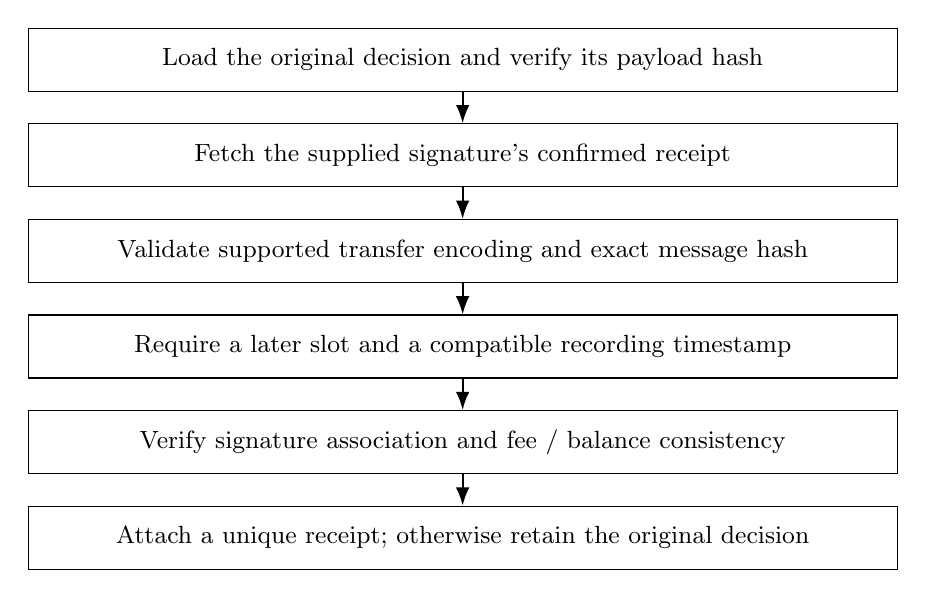
\begin{tikzpicture}[node distance=4mm,b/.style={draw,align=center,text width=108mm,minimum height=8mm,font=\small},a/.style={-{Latex},thick}]
\node[b](a){Load the original decision and verify its payload hash};
\node[b,below=of a](b){Fetch the supplied signature's confirmed receipt};
\node[b,below=of b](c){Validate supported transfer encoding and exact message hash};
\node[b,below=of c](d){Require a later slot and a compatible recording timestamp};
\node[b,below=of d](e){Verify signature association and fee / balance consistency};
\node[b,below=of e](f){Attach a unique receipt; otherwise retain the original decision};
\foreach \x/\y in {a/b,b/c,c/d,d/e,e/f}\draw[a](\x)--(\y);
\end{tikzpicture}\caption{Checks before a receipt becomes an observed outcome.}\end{figure}

\section{Experimental Setup and Test Cases}
\begin{table}[H]\centering\caption{Test inputs and expected safeguards}
\small\begin{tabularx}{\textwidth}{p{12mm}YY}\toprule ID&Scenario&Expected response\\\midrule
T01&Current label supplied to replay&Current prediction excludes that outcome\\
T02&History timestamp is in the future&Reject invalid history\\
T03&Snapshot older than one hour&Withhold ML score and request refresh\\
T04&Mainnet request with devnet history&Do not score using the wrong network\\
T05&Amount exceeds balance plus fee budget&Return the exact shortfall\\
T06&Simulation reports rent-related error&Return an actionable current-state finding\\
T07&Receipt belongs to another message&Reject outcome attachment\\
T08&Receipt predates recorded observation&Reject retrospective attachment\\
T09&No confirmed receipt is returned&Keep outcome and paid fee unknown\\
T10&Attempt to overwrite stored decision&Database trigger rejects mutation\\
T11&Unsigned input sent to signed observer&Reject unsupported signed observation\\
T12&Repeated history-refresh request&Reuse the running job rather than duplicate it\\\bottomrule\end{tabularx}\end{table}
These scenarios are grounded in the implemented tests and recorded checks. Network-dependent examples are observations from their recorded run; their outputs can change as balances and chain state change. Unit tests exercise controlled inputs so that key invariants can be repeated independently of public RPC availability.
\subsection{Local Experiment Procedure}
The verification script starts its own loopback validator and creates throwaway test accounts funded through local airdrops. It constructs an invalid transfer whose execution violates an account minimum-balance requirement. The checker observes the error. The experiment then compares a stopped candidate, ordinary preflight rejection and a deliberately forced execution failure with preflight disabled only inside the isolated test.

For the executed case, the script retrieves the confirmed receipt and compares the reported fee with the payer's before-and-after balance. The failed transfer does not deliver the requested principal, but the execution fee is observed. A valid transfer separately verifies that the sender's balance decreases by principal plus fee. The script stops the validator instance it started.

\section{Prototype / System Implementation}
The recorded integration checks include a small transfer, insufficient balance, a rent-related failure and a read-only mainnet case. The system returns current findings and, where historical inputs qualify, actual fitted-model inference. HTTP success alone is insufficient: the response content and the absence of a broadcast path are also inspected.

The presentation connects inputs, findings and the stored decision, supported by historical results and local receipts.

\section{Testing and Validation}
Targeted automated tests cover feature timing, inference, transfer-message construction, policy arithmetic and receipt integrity. The recorded verification run reports 45 passing targeted tests. This count refers to the selected project checks, not a claim about every test in the repository.
\begin{table}[H]\centering\caption{Implemented checks and recorded verification}
\small\begin{tabularx}{\textwidth}{p{35mm}YY}\toprule Area&Expected behaviour&Recorded verification\\\midrule
History maturity&Exclude current and immature outcomes&Targeted tests passed\\
Freshness and network&Withhold scores for stale or mismatched data&Targeted tests passed\\
Insufficient balance&Show amount-plus-fee shortfall&Live HTTP case verified\\
Rent constraint&Surface simulation error&Live HTTP case verified\\
Valid small transfer&Show simulation pass at checked state&Live HTTP case verified\\
Read-only operation&Do not broadcast from web checks&Targeted tests and HTTP checks\\
Receipt integrity&Reject unrelated, old or duplicate receipts&Targeted tests passed\\
Local receipt flow&Attach matching later receipt to stored decision&Local validator verification\\\bottomrule\end{tabularx}\end{table}
\subsection{Fee-Mechanism Experiment}
An isolated local validator and throwaway keys are used to compare a deliberately invalid transfer under different submission conditions. Normal preflight rejects the invalid candidate without a paid transaction fee. In a test-only path, disabling preflight allows a landed execution failure; the receipt and balance change record 5,000 lamports. A successful transfer separately checks principal-plus-fee accounting.

This experiment verifies fee behaviour and traceable outcomes. It does not establish that the ML model outperforms ordinary preflight. The local validator uses test funds and the production web flow does not bypass preflight or submit transactions.

\chapter{RESULTS, ANALYSIS AND DISCUSSION}
\section{Results}
\begin{table}[H]\centering\caption{Cold-history AP without the identity-score control}
\begin{tabular}{lrrr}\toprule Test date&Transactions&Baseline AP&Context AP\\\midrule Nov. 3&19,621&0.3193&0.3787\\Nov. 10&20,636&0.2249&0.2514\\Nov. 24&21,028&0.2052&0.2231\\Dec. 1&19,577&0.1734&0.2185\\\bottomrule\end{tabular}\end{table}
All four point estimates favour writable context, but the November 24 interval for the difference crosses zero. Results therefore do not imply an advantage in every period.
\begin{table}[H]\centering\caption{First-appearance results with the identity-score control}
\small\begin{tabularx}{\textwidth}{lrrrY}\toprule Test&Rows&Baseline AP&Context AP&AP gain, 95\% interval\\\midrule Dec. 1&17,904&0.1688&0.2004&0.0316 [0.0168, 0.0501]\\Dec. 5&19,515&0.2207&0.2393&0.0186 [0.0095, 0.0288]\\\bottomrule\end{tabularx}\end{table}
The reserved December 1 endpoint has 5.88\% failure prevalence. Its AUROC rises from 0.7288 to 0.7545. The further December 5 result also supports additional ranking signal beyond the shared identity control.
\begin{figure}[H]\centering
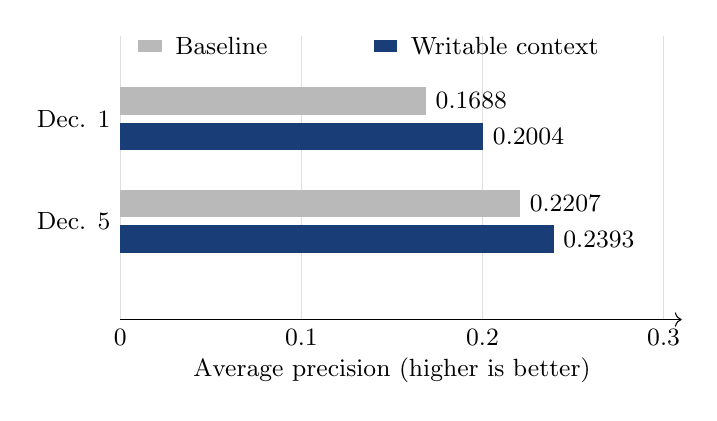
\begin{tikzpicture}[x=23cm,y=1cm,font=\small]
\foreach \v in {0,0.1,0.2,0.3}{\draw[gray!25] (\v,0)--(\v,3.6);\node[below] at (\v,0){\v};}
\draw[->] (0,0)--(.31,0);
\fill[gray!55] (0,2.6) rectangle (.1688,2.95);
\fill[institution] (0,2.15) rectangle (.2004,2.5);
\fill[gray!55] (0,1.3) rectangle (.2207,1.65);
\fill[institution] (0,.85) rectangle (.2393,1.2);
\node[left] at (0,2.55){Dec. 1};\node[left] at (0,1.25){Dec. 5};
\node[right] at (.1688,2.78){0.1688};\node[right] at (.2004,2.32){0.2004};
\node[right] at (.2207,1.48){0.2207};\node[right] at (.2393,1.02){0.2393};
\node at (.15,-.65){Average precision (higher is better)};
\fill[gray!55] (.01,3.4) rectangle (.023,3.55);\node[right] at (.025,3.48){Baseline};
\fill[institution] (.14,3.4) rectangle (.153,3.55);\node[right] at (.155,3.48){Writable context};
\end{tikzpicture}
\caption{Identity-controlled first-appearance AP on two test dates. The plot shows ranking performance, not classification accuracy.}
\end{figure}
\subsection{Fee-Policy and Local Results}
\begin{table}[H]\centering\caption{Measured local fee-mechanism outcomes}
\begin{tabularx}{\textwidth}{Y r}\toprule Local condition&Paid fee (lamports)\\\midrule Check candidate and stop&0\\Normal preflight rejects invalid candidate&0\\Force landed execution failure in isolated test&5,000\\\bottomrule\end{tabularx}\end{table}
A retrospective policy audit covers 102,443 cold-history transactions with 6,410 failures. At an assumed false-warning cost five times a failed-attempt fee, context warnings cover 107 failures and 60 successes while missing 6,303 failures. Hypothetical utility is $107-5(60)=-193$ fee units. These units are assumed costs, not measured SOL savings.

\section{Analysis}
On December 1, the AP difference is $0.2004-0.1688=0.0316$, or about 3.16 AP percentage points. Relative to the baseline AP, this is approximately an 18.7\% increase. This relative change is a ranking comparison; it must not be described as 18.7\% fewer failed transactions or an 18.7\% reduction in fees.

On December 5, the corresponding difference is approximately 0.0186. Both first-appearance intervals exclude zero under the specified paired-hour analysis. The second test has a smaller gain, which is consistent with the usefulness of context changing across sampled dates. Neither result implies correct predictions for every individual transaction.

On December 1, inherited validation thresholds yield false-positive rates of 22.66\% for the baseline and 28.65\% for the context model. Recall rises from 50.90\% to 64.48\%, but this comparison does not hold false positives constant. Brier loss worsens from 0.0967 to 0.1218. Better ranking therefore does not automatically mean better calibrated probabilities or a better warning policy.

In the interface, a displayed score such as 30.8\% is a model output for one transaction, not 30.8\% model accuracy. Whether a case is flagged depends on a threshold; judging a policy requires outcomes across many transactions and attention to both missed failures and false alarms.

\section{Discussion}
The interface displays the fraction of relevant accounts with available history so the user can see the amount of contextual coverage. A high coverage fraction means the model has earlier observations for more of those accounts. It does not imply high-quality or representative observations, and it does not guarantee confidence in the prediction.

Two models may give different scores to the same transaction because one has additional features. For the earlier example with scores 41.5\% and 30.8\%, a threshold can flag one and not the other. If the transaction succeeds, the lower score may be more consistent with that single outcome; if it fails, the higher score may be. Aggregate ranking, calibration and operating metrics are needed to judge which approach is better overall.

\section{Comparison with Existing Approaches}
The baseline and writable-context models use matched classifier settings and chronological periods. The identity-controlled comparison supplies the same learned score to both. These within-dataset comparisons isolate the added feature group. Literature methods using different targets and datasets are not claimed as directly outperformed.

\section{Significance and Implications}
The project establishes that the fitted models can be executed on constructed features, current network checks can be performed for supported transfers, and an observation can be preserved before a matching receipt is attached. The fee experiment establishes that the stage at which a transaction fails matters for fee accounting. These are separate, inspectable engineering outcomes.

The policy audit also provides an informative negative finding: the tested ranking gains do not translate automatically into favourable pooled cost utility. A useful final-year research report includes that result because it identifies the actual deployment problem. Calibrating a score, choosing a warning threshold and evaluating the cost of delaying a successful transaction are distinct from fitting the classifier.

\section{Potential Applications}
The prototype can support research inspection, prioritisation of transactions for review, and diagnosis of supported native SOL transfer problems. Balance and simulation findings can guide a user before submission. Automatic transaction blocking or economic savings require separate policy evaluation.

\chapter{CONCLUSION AND FUTURE SCOPE}
\section{Summary of Work}
HOMIE implements an end-to-end transaction-risk research system on Solana. Public records are transformed into time-respecting account features, established machine learning models are compared, and predictions are exposed through an application with live checks and traceable outcomes.

The strongest finding is that writable-account participation history adds failure-ranking signal for sampled first-appearance signers, including comparisons with a learned identity control. The project also verifies the fee mechanism and the decision-to-receipt workflow. Its results distinguish predictive ranking from probability calibration and economic benefit.

\section{Conclusions}
Writable-account history improves the reported first-appearance AP on two chronological tests with a shared identity control. The warning-policy audit shows that ranking improvement alone does not guarantee favourable cost utility.

\section{Contributions}
The project integrates chronological participation features, controlled model comparisons, a working inference interface and a decision-to-receipt workflow. A separate local experiment verifies execution-fee behaviour.

\section{Utility / Applications}
HOMIE provides an inspectable system for studying transaction failure and checking supported transfers. It makes model predictions, current network checks and later execution outcomes available as separate observations.

\section{Limitations}
The implemented system provides an inspectable ML comparison, current balance and simulation checks, and a record linking decisions to verified receipts. This is useful for studying failure risk and diagnosing supported transfer problems before submission.

The historical sample is sparse and originates from one provider. Inclusion timestamps approximate information availability rather than submission time. The selected table excludes unlanded attempts and full instruction payloads. Historical identity controls and participation features have slightly different update schedules. Live RPC sampling differs from training, and a simulation pass is state-dependent. Measured ML-driven fee savings and retry-time reductions are not established by the current experiments.

\section{Scope for Future Work}
Further work can evaluate independent data sources and periods, align identity-learning update schedules, and test cold-specific calibration under changing conditions. A prospective study should compare candidates that pass normal preflight before measuring any incremental ML benefit. Broader transaction types, authorised wallet integration and measured user task times are additional extensions. These are extensions to the completed research prototype rather than results claimed in this report.

\begingroup
\renewcommand{\bibname}{REFERENCES}
\begin{thebibliography}{99}\addcontentsline{toc}{chapter}{References}
\small\raggedright\setlength{\itemsep}{7pt}
\bibitem{accounts} Solana Foundation, ``Accounts,'' official documentation. \url{https://solana.com/docs/core/accounts}. Accessed October 16, 2026.
\bibitem{transactions} Solana Foundation, ``Transactions,'' official documentation. \url{https://solana.com/docs/core/transactions}. Accessed October 16, 2026.
\bibitem{zheng} X. Zheng, Z. Wan, D. Lo, D. Xie and X. Yang, ``Why Does My Transaction Fail? A First Look at Failed Transactions on the Solana Blockchain,'' 2025. \url{https://arxiv.org/abs/2504.18055}. DOI: 10.1145/3728943.
\bibitem{fees} Solana Foundation, ``Fees,'' official documentation. \url{https://solana.com/docs/core/fees}.
\bibitem{simulation} Solana Foundation, ``simulateTransaction,'' RPC documentation. \url{https://solana.com/docs/rpc/http/simulatetransaction}.
\bibitem{send} Solana Foundation, ``sendTransaction,'' RPC documentation. \url{https://solana.com/docs/rpc/http/sendtransaction}.
\bibitem{hgb} scikit-learn developers, ``HistGradientBoostingClassifier,'' official API documentation. \url{https://scikit-learn.org/stable/modules/generated/sklearn.ensemble.HistGradientBoostingClassifier.html}.
\bibitem{archive} SolArchive, ``SolArchive transaction dataset,'' Hugging Face, CC BY 4.0. \url{https://huggingface.co/datasets/solarchive/solarchive}. Revision specified in Chapter 4.
\bibitem{bright} M. Lu et al., ``BRIGHT -- Graph Neural Networks in Real-Time Fraud Detection,'' 2022. \url{https://arxiv.org/abs/2205.13084}.
\bibitem{friedman} J. H. Friedman, ``Greedy function approximation: A gradient boosting machine,'' \emph{The Annals of Statistics}, vol. 29, no. 5, pp. 1189--1232, 2001. \url{https://doi.org/10.1214/aos/1013203451}.
\bibitem{xgboost} T. Chen and C. Guestrin, ``XGBoost: A Scalable Tree Boosting System,'' 2016. \url{https://arxiv.org/abs/1603.02754}.
\bibitem{lightgbm} G. Ke et al., ``LightGBM: A Highly Efficient Gradient Boosting Decision Tree,'' \emph{Advances in Neural Information Processing Systems}, vol. 30, 2017. \url{https://proceedings.neurips.cc/paper_files/paper/2017/hash/6449f44a102fde848669bdd9eb6b76fa-Abstract.html}.
\bibitem{niculescu} A. Niculescu-Mizil and R. Caruana, ``Predicting Good Probabilities With Supervised Learning,'' in \emph{Proceedings of ICML}, 2005. \url{https://doi.org/10.1145/1102351.1102430}.
\bibitem{saito} T. Saito and M. Rehmsmeier, ``The Precision-Recall Plot Is More Informative than the ROC Plot When Evaluating Binary Classifiers on Imbalanced Datasets,'' \emph{PLOS ONE}, vol. 10, no. 3, e0118432, 2015. \url{https://doi.org/10.1371/journal.pone.0118432}.
\bibitem{leakage} S. Kapoor and A. Narayanan, ``Leakage and the Reproducibility Crisis in ML-based Science,'' arXiv:2207.07048, 2022. \url{https://arxiv.org/abs/2207.07048}.
\bibitem{hashing} K. Weinberger, A. Dasgupta, J. Attenberg, J. Langford and A. Smola, ``Feature Hashing for Large Scale Multitask Learning,'' 2009. \url{https://arxiv.org/abs/0902.2206}.
\bibitem{pandas} W. McKinney, ``Data Structures for Statistical Computing in Python,'' in \emph{Proceedings of the 9th Python in Science Conference}, pp. 56--61, 2010. \url{https://doi.org/10.25080/Majora-92bf1922-00a}.
\bibitem{numpy} C. R. Harris et al., ``Array programming with NumPy,'' \emph{Nature}, vol. 585, pp. 357--362, 2020. \url{https://doi.org/10.1038/s41586-020-2649-2}.
\bibitem{sklearn} F. Pedregosa et al., ``Scikit-learn: Machine Learning in Python,'' \emph{Journal of Machine Learning Research}, vol. 12, pp. 2825--2830, 2011. \url{https://jmlr.org/papers/v12/pedregosa11a.html}.
\bibitem{ap} scikit-learn developers, ``average\_precision\_score,'' API documentation. \url{https://scikit-learn.org/stable/modules/generated/sklearn.metrics.average_precision_score.html}. Accessed October 16, 2026.
\bibitem{brier} scikit-learn developers, ``brier\_score\_loss,'' API documentation. \url{https://scikit-learn.org/stable/modules/generated/sklearn.metrics.brier_score_loss.html}. Accessed October 16, 2026.
\bibitem{sgd} scikit-learn developers, ``SGDClassifier,'' API documentation. \url{https://scikit-learn.org/stable/modules/generated/sklearn.linear_model.SGDClassifier.html}. Accessed October 16, 2026.
\bibitem{isotonic} scikit-learn developers, ``IsotonicRegression,'' API documentation. \url{https://scikit-learn.org/stable/modules/generated/sklearn.isotonic.IsotonicRegression.html}. Accessed October 16, 2026.
\bibitem{fastapi} FastAPI contributors, ``FastAPI,'' official documentation. \url{https://fastapi.tiangolo.com/}. Accessed October 16, 2026.
\bibitem{blockhash} Solana Foundation, ``getLatestBlockhash,'' official documentation. \url{https://solana.com/docs/rpc/http/getlatestblockhash}. Accessed October 16, 2026.
\bibitem{feequote} Solana Foundation, ``getFeeForMessage,'' official documentation. \url{https://solana.com/docs/rpc/http/getfeeformessage}. Accessed October 16, 2026.
\bibitem{balance} Solana Foundation, ``getBalance,'' official documentation. \url{https://solana.com/docs/rpc/http/getbalance}. Accessed October 16, 2026.
\bibitem{getblock} Solana Foundation, ``getBlock,'' official documentation. \url{https://solana.com/docs/rpc/http/getblock}. Accessed October 16, 2026.
\bibitem{gettransaction} Solana Foundation, ``getTransaction,'' official documentation. \url{https://solana.com/docs/rpc/http/gettransaction}. Accessed October 16, 2026.
\bibitem{sqlite} SQLite developers, ``CREATE TRIGGER,'' SQL language documentation. \url{https://www.sqlite.org/lang_createtrigger.html}. Accessed October 16, 2026.
\end{thebibliography}
\endgroup
\appendix
\chapter{REPRODUCIBILITY AND USER GUIDE}

\section{Project components}
The active research implementation is under \texttt{research/solana/ml}. The current web application uses \texttt{webapp/backend/replay.py}. Older project prototypes remain in the repository; they are not the implementation described by this report. The model artifact and processed features must exist before live inference can run.
\begin{table}[H]\centering\caption{Evidence and implementation locations}
\small\begin{tabularx}{\textwidth}{p{38mm}Y}\toprule Purpose&Location relative to the project root\\\midrule
Research scripts&\path{research/solana/ml/}\\
Local fee verification&\path{research/solana/fee_proof/}\\
Live feature construction&\path{webapp/backend/live_history.py}\\
Transfer checking&\path{webapp/backend/transfer_check.py}\\
Decision and receipt store&\path{webapp/backend/prospective.py}\\
Saved experimental reports&\path{docs/results/}\\
Model and derived data&\path{data/processed/solana_ml/}\\\bottomrule\end{tabularx}\end{table}
\section{Running the application}
From the repository root, activate the project Python environment and use the documented model export after preparing the processed training data. Collect a recent history for the desired network. Start the current FastAPI application with:
\begin{quote}\small\ttfamily
.venv/bin/python -m uvicorn\\
webapp.backend.replay:app --host 127.0.0.1 --port 8430
\end{quote}
The command is shown over two lines for readability; enter it as one shell command. Open \url{http://127.0.0.1:8430/live}. Refresh historical inputs if the page reports a stale snapshot. Public RPC availability affects collection and live checks.
\section{Suggested demonstration sequence}
\begin{enumerate}
\item Open the historical replay and explain the missing-history problem.
\item Select a transaction, compare the two models and reveal its recorded outcome.
\item Open the live checker and enter a supported transfer on the intended network.
\item Explain the balance, quoted fee and simulation result before the experimental ML score.
\item Inspect the saved observation and its model/history provenance.
\item Show the local fee receipts and the chronological research results.
\end{enumerate}
This sequence demonstrates both the research pipeline and the implemented system. A live model score is not presented as a new evaluated accuracy figure, and the absence of submission is not counted as a measured saving.
\section{Terms used during the viva}
\begin{description}[style=nextline]
\item[Execution failure] A transaction with a recorded unsuccessful execution outcome.
\item[Cold history] No matured primary-signer outcome available in the sampled history.
\item[First appearance] The signer's first observed occurrence in the replay.
\item[Shared-account context] Earlier participation of accounts referenced by the current transaction.
\item[Baseline] The comparison model before adding writable-history summaries.
\item[Ablation] A controlled comparison where a feature group is added or removed.
\item[Calibration] Agreement between numerical scores and observed event frequencies.
\item[False positive] A successful transaction incorrectly flagged by a warning policy.
\item[Preflight] Checks associated with submission that may reject a candidate before it is sent for execution.
\item[Receipt] A retrieved record of a transaction's observed execution outcome and fee.
\end{description}
\section{Short explanation of the contribution}
HOMIE asks whether a transaction can be assessed when its signer has no usable history. It learns from earlier transactions involving other accounts used by that operation. The project compares models fairly over time, finds additional ranking signal in the studied data, and implements a system that displays predictions alongside current transfer checks and recorded outcomes.

\end{document}
